\documentclass[12pt, oneside]{report}

\usepackage[left=2.5cm, top=2.5cm, bottom=2.5cm, right=2.5cm]{geometry}

\usepackage[backend=bibtex,style=verbose-trad2]{biblatex}
\bibliography{bibliography}

\usepackage[utf8]{inputenc}
\usepackage[T1]{polski}
\usepackage[polish,english]{babel}
\selectlanguage{polish}
\usepackage{svg}
\usepackage{pdfpages}

\begin{document}
\thispagestyle{empty}
\begin{titlepage}
    \begin{center}

           \Large
	\textbf{Uniwersytet Jagielloński w Krakowie}\vspace{0.2cm}\\ Wydział Fizyki, Astronomii i Informatyki Stosowanej
               \vspace*{1cm}

         \vspace{3cm}
         \Large
          \textbf{Jakub Wida}\\\vspace{0.5cm}
         \normalsize Nr albumu: 1113470\\
             \vspace{2cm}
        \Huge
        \textbf{Losowe upakowania układów złożonych z dysków z wykorzystaniem kart graficznych}

        \vspace{1.5cm}
        \normalsize
        Praca magisterska\\
        na kierunku Informatyka Stosowana\\ \vspace{0.15cm}

        \vfill
        \vspace{2cm}
       \begin{minipage}{1\textwidth}
\begin{flushright}
Praca wykonana pod kierunkiem\\
dr. hab. Michała Cieśli\\
z Zakładu Fizyki Statystycznej
\end{flushright}
\end{minipage}

        \vspace{2cm}
        \begin{center}
      Kraków 2019
        \end{center}
    \end{center}
\end{titlepage}

\newpage
 \thispagestyle{empty}
\vspace{2.5cm}
\begin{flushleft}
\large \textbf{Oświadczenie autora pracy}\vspace{0.6cm}\\
\end{flushleft}

\noindent Świadom odpowiedzialności prawnej oświadczam, że niniejsza praca dyplomowa została napisana przeze mnie samodzielnie i nie zawiera treści uzyskanych w sposób niezgodny z obowiązującymi przepisami.\\

\noindent Oświadczam również, że przedstawiona praca nie była wcześniej przedmiotem procedur związanych z uzyskaniem tytułu zawodowego w wyższej uczelni.
\vspace{2cm}
\begin{center}
\begin{tabular}{lr}
................................~~~~~~~~~~~~~~~~~~~~~~~~~~~~~~~~~~~~~~&
.......................................... \\
{~~~~Kraków, dnia} & {Podpis autora pracy~~~~}
\end{tabular}
\end{center}
\vspace{5cm}
\begin{flushleft}
\large \textbf{Oświadczenie kierującego pracą}
\end{flushleft}

\noindent Potwierdzam, że niniejsza praca została przygotowana pod moim kierunkiem i~kwalifikuje się do przedstawienia jej w postępowaniu o nadanie tytułu zawodowego.
\vspace{2cm}
\begin{center}
\begin{tabular}{lr}
................................~~~~~~~~~~~~~~~~~~~~~~~~~~~~~~~~~~~~~~&
............................................ \\
{~~~~Kraków, dnia} & {Podpis kierującego pracą~~}
\end{tabular}
\end{center}
\vfill


%INTRODUCTION ====================================================

\selectlanguage{english}

\chapter{Introduction}
{\bf TODO make this at the end, when all else is done}


%TABLE OF CONTENTS ====================================================

\tableofcontents
\newpage

%ACTUAL THESIS: INTRO ====================================================

%2-4 pages
\chapter{Problem Overwiev}
\section {Random Sequential Adsorbtion}

Random Sequential Adsorbtion is a stochastic process, that can be described as sequential insertion of given shapes onto an empty, limited euclidean space. The shapes are inserted with random position, and in such a way, that if the shape is colliding with an already inserted shape, it is then rejected in the process. The shapes and the space may be defined as having one or more dimensions, with any kind of inserted shape type. The shapes may be generated with random coordinates within given dimensions, as well as random rotation - although this may be optional.\autocite[1]{zhang}\autocite[1]{feder}

\subsection {Shape Types}

The inserted shape that were previously studied include rectangles, squares and other polygons, cubes and hypercubes. Also, the most basic shape usually investigated is a sphere - up to eight dimensions. Other studies involved spheroids, hyperdisks and, what is going to be further investigated in this thesis, disk polymers, or simply two dimensional groups of disks. In case of non spherical shapes, the shape angle can be randomly generated.\autocite[1]{zhang}

\subsection {Applications}

The Random Sequential Adsorbtion can be applied to multiple problems. The process as well as the generated shapes can be used to model a variety of phenomena. These include the ion implantation in semiconductors, structure of the cement paste, particles in cell membranes, protein adsorption and settlement of animal territories.\autocite[1]{zhang} In general, it can be used to model tightly - but still randomly - packed particles.
\newline

A significant example is the Poisson Disk Sampling, which is a process of selection of points in subdomain, in such a way that within a given distance from the selected point, no other are taken. This distribution is used in computer graphics for rendering, texture generation, and more. In ray tracing, it is used to create soft shadow, motion blur and the depth of field. In physics, it can be used for mesh generation, interpolation and process modeling. In some cases, the generated meshes have improved quality and are generated more robustly. \autocite[1]{ebeida}

\subsection {Challenges}

While the principle behind RSA algorithms is simple, the execution of it's naive implementations will commonly lead to problems. As the figures are randomly generated and inserted to the area, the probability of rejection of said shape will grow with the saturation of the system. In simpler words, the more figures are already inserted, the more likely it is that a new one will overlap a pre-existing one, which leads to long execution times and uncertain end conditions. The goal of many approaches is to propose an algorithm that will be able to quickly generate shapes within given space, and have clear end conditions signifying a fully saturated state.

\section {Thesis Goals}

This thesis focuses on one particular subset of RSA, namely, the generation of polydisks in two dimensional space. It's goal was to create an algorithm that would take advantage of great degree of parallelization available through using the GPU. A pre-existing algorithm developed by dr. hab. Michał Cieśla enables quick sequential or thread-level parallel generation of polydisks in a 2D area. Such algorithm can be used to simulate the packings of particles on a surface; Which itself is usefull in physics and material research.\autocite[1]{ciesla}

%ACTUAL THESIS: ALGORITHM OVERWIEV ====================================================

%5-15 pages
\chapter{Proposed Algorithm}

\section {Voxel-Based Algorithm}

The basic algorithm used in multiple RSA applications involves the use of voxels. The voxels are defined as subspaces of the saturated area, which cover it entirely. After one or more shapes are inserted, the voxels may be removed if within them no more figures can be inserted. Developing an algorithm for "voxel rejection" is the main concern of those undertakings. Only within the non-removed voxels the figures can be generated. After inserting more figures, if the voxels are not rejected or the figures are rejected too commonly - the voxels are split into smaller voxels to be able to further reject them. If all voxels are removed, the system is saturated. An example of such algorithm, using the two dimensional circles as shapes is demonstrated in the figure \ref{VoxelCircleRSApdf}.

\begin{figure}
	\label{VoxelCircleRSApdf}
  \centering
	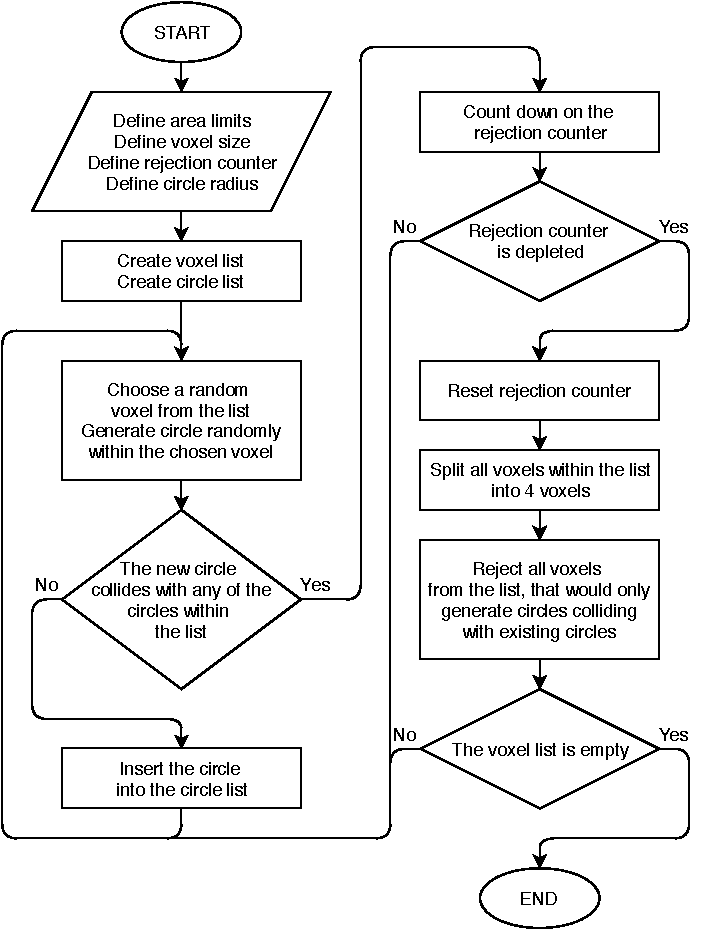
\includegraphics{Images/2dCircleRSA/VoxelCircleRSA.pdf}
  \caption{The flowchart of simple 2D RSA algorithm, using circles}
\end{figure}

\section {Sequential Algorithm}
	%describe basic algorithm, from dr.hab. Ciesla works



\section {Parallel Application}
	%describe changes to basic algorithm, provide complete outline of target, parallel algorithm
\subsection{Block Graph}
	%draw a block graph
\section {Implementation}
	%write in general about implementing, challenges etc
\subsection{PyCuda}
	%write about language specifics, improvements over raw CUDA
\subsection{Visualisation}
	%about pyplot - shortly
\subsection{Summary}
	%stuff in general

{\bf TODO unfinished, do in near future}

%ACTUAL THESIS: RESULTS INVESTIGATION ====================================================

%15-25 pages - due to multiple pictures
\chapter{Results Examination}
\section{Performance Evaluation}
	%describe importance of performance evaluation
	%describe the algorithm runner, and hot it works
\subsection{Parameter Influence over Performance}
\subsection{Shape Influence over Performance}
{\bf TODO unfinished, do later}

%ACTUAL THESIS: BIBLIOGRAPHY ====================================================

\newpage
\printbibliography

\end{document}
